\def\mytitle{IDE ASSIGMNMENT}
\def\myauthor{MOHAMMAD ADHIL}
\def\contact{20211a04d8@bvrit.ac.in}
\def\mymodule{Future Wireless Communications (FWC)}
\documentclass[journal,12pt,twocolumn]{IEEEtran}
\usepackage{setspace}
\usepackage{gensymb}
\usepackage{xcolor}
\usepackage{caption}
\usepackage[hyphens,spaces,obeyspaces]{url}
\usepackage[cmex10]{amsmath}
\usepackage{mathtools}
\singlespacing
\usepackage{amsthm}
\usepackage{mathrsfs}
\usepackage{txfonts}
\usepackage{stfloats}
\usepackage{cite}
\usepackage{cases}
\usepackage{subfig}
\usepackage{longtable}
\usepackage{multirow}
\twocolumn
\usepackage{graphicx}
\graphicspath{{./images/}}
\usepackage[colorlinks,linkcolor={black},citecolor={blue!80!black},urlcolor={blue!80!black}]{hyperref}
\usepackage[parfill]{parskip}
\usepackage{lmodern}
\usepackage{tikz}
\usepackage{circuitikz}
\usepackage{karnaugh-map}
\usepackage{pgf}
\usepackage[hyphenbreaks]{breakurl}
\usepackage{tabularx}
\usetikzlibrary{calc}
\renewcommand*\familydefault{\sfdefault}
\usepackage{watermark}
\usepackage{lipsum}
\usepackage{xcolor}
\usepackage{listings}
\usepackage{float}
\usepackage{titlesec}
\DeclareMathOperator*{\Res}{Res}
\renewcommand\thesection{\arabic{section}}
\renewcommand\thesubsection{\thesection.\arabic{subsection}}
\renewcommand\thesubsubsection{\thesubsection.\arabic{subsubsection}}
\renewcommand\thesectiondis{\arabic{section}}
\renewcommand\thesubsectiondis{\thesectiondis.\arabic{subsection}}
\renewcommand\thesubsubsectiondis{\thesubsectiondis.\arabic{subsubsection}}
\titlespacing{\subsection}{1pt}{\parskip}{3pt}
\titlespacing{\subsubsection}{0pt}{\parskip}{-\parskip}
\titlespacing{\paragraph}{0pt}{\parskip}{\parskip}
\newcommand{\figuremacro}[5]{
    \begin{figure}[#1]
        \centering
\begin{figure}
            \centering
            \includegraphics[width=0.5\linewidth]{led.webp}
            \caption{Enter Caption}
            \label{fig:enter-label}
        \end{figure}
        \includegraphics[width=#5\columnwidth]{#2}
        \caption[#3]{\textbf{#3}#4}
        \label{ig:#2}
    \end{figure}
}
\lstset{
frame=single, 
breaklines=true,
columns=fullflexible
}
%\thiswatermark{\centering \put(400,-128.0){\includegraphics[scale=0.3]{logo}} }
\title{\mytitle}
\author{\myauthor\hspace{1em}\\\contact\\IITH\hspace{0.5em}-\hspace{0.6em}\mymodule}
\date{20-12-2022}
\def\inputGnumericTable{}                                 %%
\lstset{
%language=C,
frame=single, 
breaklines=true,
columns=fullflexible
}
 \begin{document}
%
\theoremstyle{definition}
\newtheorem{theorem}{Theorem}[section]
\newtheorem{problem}{Problem}
\newtheorem{proposition}{Proposition}[section]
\newtheorem{lemma}{Lemma}[section]
\newtheorem{corollary}[theorem]{Corollary}
\newtheorem{example}{Example}[section]
\newtheorem{definition}{Definition}[section]
%\newtheorem{algorithm}{Algorithm}[section]
%\newtheorem{cor}{Corollary}
\newcommand{\BEQA}{\begin{eqnarray}}
\newcommand{\EEQA}{\end{eqnarray}}
\newcommand{\define}{\stackrel{\triangle}{=}}
\bibliographystyle{IEEEtran}
\vspace{3cm}
\maketitle
\tableofcontents
  \section{question}
     In the circiut shown below , assume that the comparators are ideal and all components have zero propagation delay . In one period of the input signal Vin=6sin(wt),the fraction of the time which the output OUT is in login state HIGH is 
     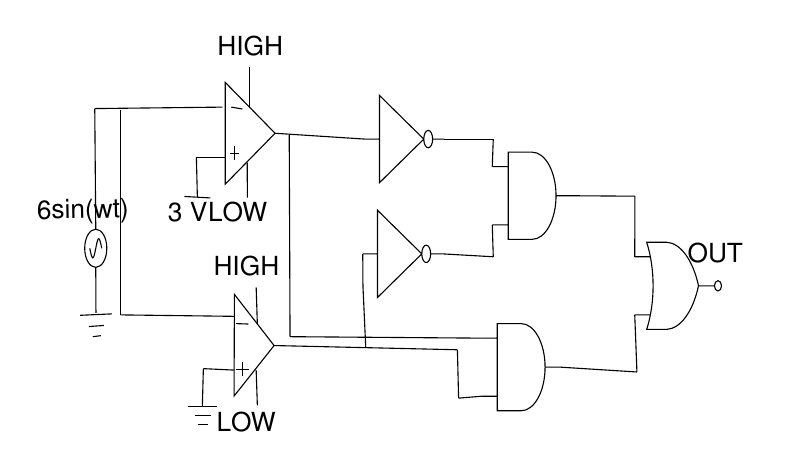
\begin{tikzpicture}[x=0.45pt,y=0.35pt,yscale=-1.5,xscale=0.8]
\tikzset{every picture/.style={line width=0.75pt}} %set default line width to 0.75pt        
%Straight Lines [id:da497014729381388] 
\draw    (140,132.6) -- (169,132.6) ;
%Flowchart: Extract [id:dp3321780746660581] 
\draw   (219,116) -- (169,151) -- (169,81) -- cycle ;
%Straight Lines [id:da17793857448296313] 
\draw    (38,99) -- (166,98) ;
%Straight Lines [id:da9757576729769633] 
\draw    (38,99) -- (39,182) ;
%Straight Lines [id:da772216831020951] 
\draw    (64,100) -- (64,241) ;
%Straight Lines [id:da17160688891184805] 
\draw    (140,132.6) -- (141,160) ;
%Flowchart: Extract [id:dp1753151070852037] 
\draw   (218,262.1) -- (177.82,296.89) -- (178.18,226.9) -- cycle ;
%Straight Lines [id:da8490718483620778] 
\draw    (64,241) -- (178,242) ;
%Straight Lines [id:da2131290241855488] 
\draw    (147,278) -- (146,304) ;
%Straight Lines [id:da06754998827437309] 
\draw    (147,278) -- (178,279) ;
%Straight Lines [id:da6585658480786443] 
\draw    (128,159.5) -- (154,160.5) ;
%Straight Lines [id:da38485782506888055] 
\draw    (131.5,304) -- (139.2,304) -- (160.5,304) ;
%Straight Lines [id:da9940160044670818] 
\draw    (219,116) -- (309,120) ;
%Shape: Not/Inverter Gate [id:dp6645899938254611] 
\draw   (323.81,90) -- (368.26,120) -- (323.81,150) -- (323.81,90) -- cycle (309,120) -- (323.81,120) (377.15,120) -- (389,120) (368.26,120) .. controls (368.26,116.69) and (370.25,114) .. (372.7,114) .. controls (375.16,114) and (377.15,116.69) .. (377.15,120) .. controls (377.15,123.31) and (375.16,126) .. (372.7,126) .. controls (370.25,126) and (368.26,123.31) .. (368.26,120) -- cycle ;
%Shape: Not/Inverter Gate [id:dp5203526386809565] 
\draw   (321.81,169) -- (366.26,199) -- (321.81,229) -- (321.81,169) -- cycle (307,199) -- (321.81,199) (375.15,199) -- (387,199) (366.26,199) .. controls (366.26,195.69) and (368.25,193) .. (370.7,193) .. controls (373.16,193) and (375.15,195.69) .. (375.15,199) .. controls (375.15,202.31) and (373.16,205) .. (370.7,205) .. controls (368.25,205) and (366.26,202.31) .. (366.26,199) -- cycle ;
%Shape: And Gate [id:dp9113043452641065] 
\draw   (453,129) -- (477,129) .. controls (490.25,129) and (501,142.44) .. (501,159) .. controls (501,175.56) and (490.25,189) .. (477,189) -- (453,189) -- (453,129) -- cycle (437,139) -- (453,139) (437,179) -- (453,179) (501,159) -- (517,159) ;
%Straight Lines [id:da5047558236731997] 
\draw    (389,120) -- (438,120) ;
%Straight Lines [id:da7853309017572672] 
\draw    (438,120) -- (437,139) ;
%Straight Lines [id:da09581339031746183] 
\draw    (437,179) -- (438,201) ;
%Straight Lines [id:da16150015131708795] 
\draw    (233.2,117.3) -- (234,256) ;
%Straight Lines [id:da3982360427353082] 
\draw    (218,262.1) -- (402,265) ;
%Straight Lines [id:da7763866390601679] 
\draw    (307.2,221.3) -- (310,263.55) ;
%Shape: And Gate [id:dp6929958094484654] 
\draw   (442,247) -- (466,247) .. controls (479.25,247) and (490,260.44) .. (490,277) .. controls (490,293.56) and (479.25,307) .. (466,307) -- (442,307) -- (442,247) -- cycle (426,257) -- (442,257) (426,297) -- (442,297) (490,277) -- (506,277) ;
%Straight Lines [id:da5339653129723407] 
\draw    (234,256) -- (426,257) ;
%Straight Lines [id:da3839391248130781] 
\draw    (307,199) -- (307.2,221.3) ;
%Straight Lines [id:da6726109915230507] 
\draw    (387,199) -- (438,201) ;
%Straight Lines [id:da40951430114554754] 
\draw    (402,265) -- (403.2,298.3) ;
%Straight Lines [id:da9775921532117686] 
\draw    (403.2,298.3) -- (426,297) ;
%Flowchart: Connector [id:dp8541564806415127] 
\draw   (27.9,195.15) .. controls (27.9,187.89) and (32.87,182) .. (39,182) .. controls (45.13,182) and (50.1,187.89) .. (50.1,195.15) .. controls (50.1,202.41) and (45.13,208.3) .. (39,208.3) .. controls (32.87,208.3) and (27.9,202.41) .. (27.9,195.15) -- cycle ;
%Shape: Sine Wave Form [id:dp42157572682524824] 
\draw   (33,195.15) .. controls (35.44,203.92) and (36.59,203.96) .. (39,195.15) .. controls (41.41,186.34) and (42.54,186.28) .. (45,195.15) ;
%Shape: Or Gate [id:dp7839680372805569] 
\draw   (592,191) -- (612,191) .. controls (625.95,191.54) and (638.42,203.23) .. (644,221) .. controls (638.42,238.77) and (625.95,250.46) .. (612,251) -- (592,251) .. controls (600.57,232.44) and (600.57,209.56) .. (592,191) -- cycle (580,201) -- (596,201) (580,241) -- (596,241) (644,221) -- (660,221) ;
%Straight Lines [id:da1579523714650295] 
\draw    (517,159) -- (580.2,159.3) ;
%Straight Lines [id:da6248594806976522] 
\draw    (506,277) -- (582.2,280.3) ;
%Straight Lines [id:da07782234715989711] 
\draw    (580.2,159.3) -- (580,201) ;
%Straight Lines [id:da20731054042333286] 
\draw    (580,241) -- (582.2,280.3) ;
%Straight Lines [id:da4591115076560359] 
\draw    (193.2,70.3) -- (193.2,98.3) ;
%Straight Lines [id:da9614915073120633] 
\draw    (191,136) -- (191.2,160.3) ;
%Straight Lines [id:da6267154334794827] 
\draw    (200,279) -- (201.2,303.3) ;
%Straight Lines [id:da7013095252421617] 
\draw    (200,222) -- (201.2,247.3) ;
%Straight Lines [id:da505762670676958] 
\draw    (141.2,316.3) -- (151.2,316.3) ;
%Straight Lines [id:da5523950339641612] 
\draw    (175,98) -- (186.2,99.3) ;
%Straight Lines [id:da3727188903283414] 
\draw    (138.2,310.3) -- (154.2,310.3) ;
\draw   (174,129.65) -- (183.2,129.65)(178.6,125) -- (178.6,134.3) ;
\draw   (180,278.3) -- (193.2,278.3)(186.6,273.3) -- (186.6,283.3) ;
%Straight Lines [id:da6667775045429274] 
\draw    (180,247) -- (192.2,247.3) ;
%Shape: Circle [id:dp7754800448867729] 
\draw   (660,221) .. controls (660,219.04) and (661.59,217.45) .. (663.55,217.45) .. controls (665.51,217.45) and (667.1,219.04) .. (667.1,221) .. controls (667.1,222.96) and (665.51,224.55) .. (663.55,224.55) .. controls (661.59,224.55) and (660,222.96) .. (660,221) -- cycle ;
%Straight Lines [id:da3040090400300808] 
\draw    (39,208.3) -- (39.2,239.6) ;
%Straight Lines [id:da6746368970911716] 
\draw    (23.2,241.3) -- (55.2,240.3) ;
%Straight Lines [id:da7013568848674232] 
\draw    (32,249) -- (47.2,248.3) ;
%Straight Lines [id:da40668201779662905] 
\draw    (36,256) -- (44.2,255.3) ;
% Text Node
\draw (199.7,56.16) node  [rotate=-359.96] [align=left] {\begin{minipage}[lt]{27.88pt}\setlength\topsep{0pt}
HIGH
\end{minipage}};
% Text Node
\draw (190.6,170.15) node   [align=left] {\begin{minipage}[lt]{28.02pt}\setlength\topsep{0pt}
LOW
\end{minipage}};
% Text Node
\draw (201.78,207.75) node   [align=left] {\begin{minipage}[lt]{32.1pt}\setlength\topsep{0pt}
HIGH
\end{minipage}};
% Text Node
\draw (200.1,314.75) node   [align=left] {\begin{minipage}[lt]{28.7pt}\setlength\topsep{0pt}
LOW
\end{minipage}};
% Text Node
\draw (669.1,198.75) node   [align=left] {\begin{minipage}[lt]{25.98pt}\setlength\topsep{0pt}
OUT
\end{minipage}};
% Text Node
\draw (12.13,170) node  [rotate=-358.82] [align=left] {\begin{minipage}[lt]{23.22pt}\setlength\topsep{0pt}
6sin(wt)
\end{minipage}};
% Text Node
\draw (146.6,170.65) node   [align=left] {\begin{minipage}[lt]{25.3pt}\setlength\topsep{0pt}
3 V
\end{minipage}};
\end{tikzpicture}
     \section{Components}
     \begin{tabularx}{0.4\textwidth} { 
  | >{\centering\arraybackslash}X 
  | >{\centering\arraybackslash}X 
  | >{\centering\arraybackslash}X
  | >{\centering\arraybackslash}X | }
\hline
\textbf{Component}& \textbf{Values} & \textbf{Quantity}\\
\hline
Arduino & UNO & 1 \\  
\hline
JumperWires & M-F &4 \\ 
\hline
Resistance & 220-ohms & 3\\
\hline
     \end{tabularx}
     \section{led connection}
 \begin{figure}
\centering
\includegraphics[width=\columnwidth]{figs/img1.jpg}
\caption{led}
\label{fig:img1}
\end{figure}
\section{Implementation}
  \begin{tabularx}{0.46\textwidth} { 
  | >{\centering\arraybackslash}X 
  | >{\centering\arraybackslash}X  | }
\hline
\textbf{Arduino PIN} & \textbf{lcd } \\ 
\hline
D2 & led 1 \\
\hline
D3 & led 2 \\
\hline
D8 & led 3  \\
\hline
GND & LED GRD \\
\hline
\end{tabularx}
\begin{center}
    Connections
\end{center}
\paragraph{Procedure}
    
    1. Connect the circuit as per the above table.\\
     
    2. Connect  the led to arduino\\
\pagebreak

     3. XOR GATE thruth table\\
     
    \begin{tabularx}{0.4\textwidth} { 
  | >{\centering\arraybackslash}X 
  | >{\centering\arraybackslash}X 
  | >{\centering\arraybackslash}X
  | >{\centering\arraybackslash}X | }
\hline
\textbf{A}& \textbf{B} & \textbf{OUTPUT}\\
\hline
0 & 0 & 1 \\  
\hline
0 & 1 &0\\ 
\hline
1 & 0 & 0\\
\hline
1 & 1 & 1\\
\hline
     \end{tabularx}

 \begin{figure}
\centering
\includegraphics[width=\columnwidth]{figs/img2.jpg}
\caption{Arduino connection with led}
\label{fig:img2}
\end{figure}
 \begin{tabularx}{0.75\textwidth} { 
  | >{\centering\arraybackslash}X |}
  \hline
 https://github.com/adhil2003/fwc\\/blob/main/platformio/code/code.cpp\\
  \hline
\end{tabularx}
    \section{LED OUTPUT}
 \bibliographystyle{ieeetr}
\end{document}
